\documentclass[12pt]{article}

\usepackage[dvips,letterpaper,margin=0.75in,bottom=0.5in]{geometry}
\usepackage{cite}
\usepackage{slashed}
\usepackage{graphicx}
\usepackage{amsmath}

\begin{document}

\section{Introduction}

In this lab, we will use a PID (Proportional, Integral, and Derivative)
algorithm, implemented on an Arduino microprocessor, to maintain an aluminum
block at a constant temperature.  The temperature is measured using a
thermistor, a device for which the resistance varies consistently with
temperature.  The active part of the temperature control is a thermoelectric
(TE) device, which moves heat away or toward a heat reservoir depending on the
magnitude and direction of the applied current.  This lab is based on the
exercise described in Chapter 12 and Appendix I of ``Labview for Scientists and
Engineers'' by Essic (available for further reference in the lab).

\section{Safety}

\begin{itemize}
\item The thermoelectric device can get very hot or cold.  DO NOT TOUCH unless your instructor tests it first.

\item The transitors and heat sinks can get very hot.  DO NOT TOUCH.

\item Whenever the dual 3 A power supplies are powered, keep an eye on the
  current monitors.  Only one supply should be powering the circuit at a time.
  If they both are drawing current, something has gone wrong, and you are
  driving current through both transistors...  You also should not draw more
  than 2 A.
\end{itemize}

\section{Thermistor}

\begin{figure}[ht]
\begin{center}
{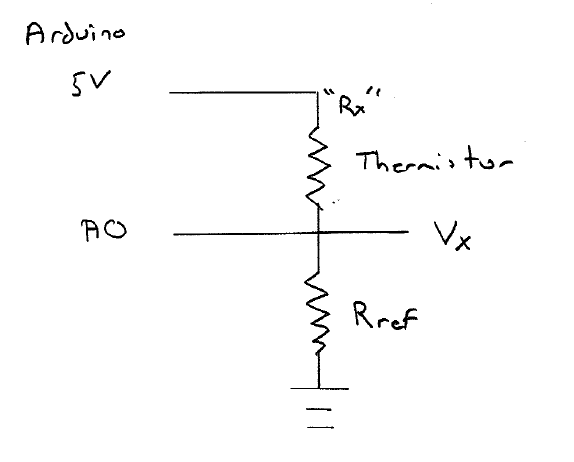
\includegraphics[width=0.70\textwidth]{figs/divider.png}}
\end{center}
\caption{\label{fig:divider} The voltage divider circuit.}
\end{figure}

You will probably be wondering wether or not your aluminum block is hot or cold,
and will therefore be tempted to touch it.  So let's quickly give you an
alternative!  First measure the resistance of the thermistor (which is connected
across the two bus terminals labeled ``Rx'' on your Thermoelectric module)
directly with your digital multimeter (DMM).  You should measure something
around $11~{\rm k\Omega}$.

Next build the voltage divider (See Fig.~\ref{fig:divider}) between the 5 volts
and ground {\em on your Arduino protoboard} using a reference resistance of
$10~{\rm k\Omega}$.  With the Arduino powered (no sketch needed yet) confirm
with your DMM that you measure a voltage of about 2.4 V across the reference
resistor.  This is consistent with what you would expect for a voltage divider:
\begin{displaymath}
\frac{V_x}{V_0} = \frac{R_x}{R_x + R_{\rm ref}}.
\end{displaymath}

Next, with the voltage across the reference resistor supplied to Arduino analog
input A0, run the ``Simple Thermometer'' Arduino sketch available from the
course smart site.  With a serial monitor open, you should see the Arduino
reporting the voltage $V_x$ (our proxy for the temperature) consistent with what
you measured with the DMM across the references resistor.

In principle, we could calibrate this voltage to the actual temperature, but we
do not have time!  So instead we will just use the voltage directly in the PID
and control algorithm.  Keep in mind that a voltage of about $2.4 V$ is room
temperature, while more than $3 V$ is noticably hot, and less than $2 V$ is
noticably cold.  DO NOT TOUCH THE ALUMINUM BLOCK unless your instructor checks
it for you first!

\section{Diffential Amplifier}

The Arduino PWM outputs are between 0 and 5~V.  To control the TE, we need to
send a voltage level between $-9~{\rm V}$ and $+9~{\rm V}$.  To make this
conversion, we'll construct a differential amplifier, which outputs a voltage
proptional to its {\em two} input voltage levels: $V_{\rm out} = G * (V_+ -
V_i)$.  To set a positive output voltage, the Arduino sets $V_+$ to a positive
value and $V_-$ to zero.  To set a negative output voltage, the Arduino sets
$V_-$ to a positive value and $V_+$ to zero.  No negative input voltages are
needed!

\begin{figure}[htb]
\begin{center}
{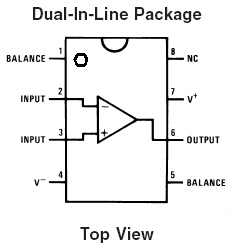
\includegraphics[width=0.30\textwidth]{figs/LF411.jpg}}
\end{center}
\caption{\label{fig:lf411} The LF411 Op Amp.}
\end{figure}

\begin{figure}[htb]
\begin{center}
{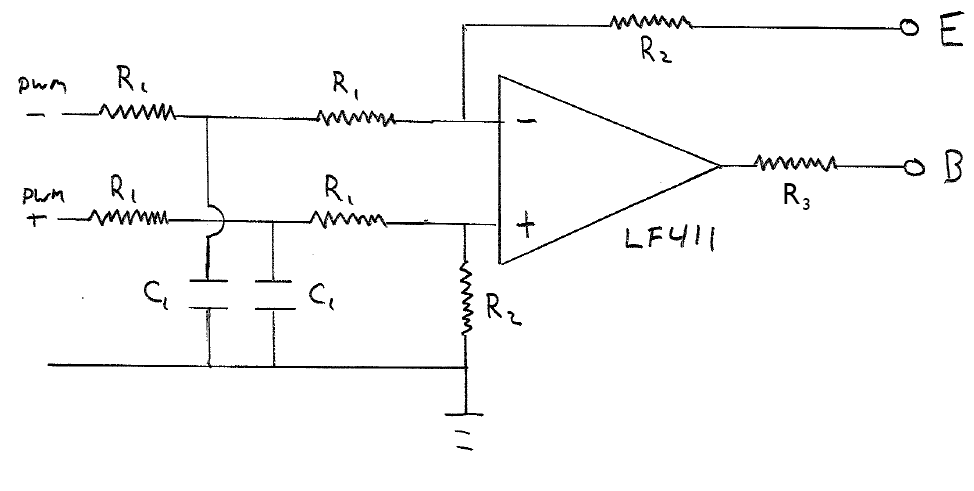
\includegraphics[width=0.90\textwidth]{figs/circuit.png}}
\end{center}
\caption{\label{fig:circuit} The differential amplifier circuit.}
\end{figure}


We will build our differential amplifier around the LF411 Op Amp shown in the
Fig.~\ref{fig:lf411}.  Built the circuit detailed in Fig.~\ref{fig:circuit}
based using the component values in Table~\ref{tbl:bom}.  {\em Do not connect
  the TE module yet!} Note that for this differential amplifier to have
symmetric gain for positive and negative signals, the feedback resistor has the
same value as the grounding resistor: $R_2$.  Also note that, though not shown
in the diagram to avoid clutter, you will have to hookup the LF411 to power
supplied by your lab proto-board.  PRO TIP: for initial debugging, adjust your
supply voltages on your protoboard to a low value still adequate to operate the
device: 6 volts.  (After things are working reliably, you will adjust these to 9
volts for full power later.)

\begin{table}[htb]
\begin{center}
\caption{\label{tbl:bom} Components} 
\vskip 1cm
\begin{tabular}{ll}
$R_1$ & $10~{\rm k\Omega}$ \\
$R_2$ & $22~{\rm k\Omega}$ \\
$R_3$ & $470~{\rm \Omega}$ \\
$C_1$  & $10~{\rm \mu F}$ (or $4.7~{\rm \mu F}$) \\ 
\end{tabular}
\end{center}
\end{table}

\begin{figure}[htb]
\begin{center}
\begin{tabular}{cc}
{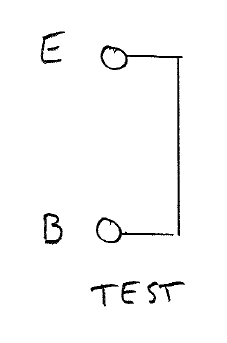
\includegraphics[height=0.30\textheight]{figs/test.png}} & 
{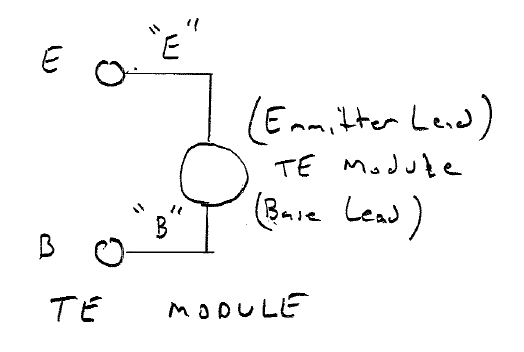
\includegraphics[height=0.30\textheight]{figs/te.png}} \\
(a) & (c) \\
\end{tabular}
\end{center}
\caption{\label{fig:feedback} Two alternatives for closing the feedback loop.  For initial testing, we do not use the TE module and close the feedback loop with the short circuit (a).  After testing, we'll connect the TE module as shown in (b) and described below.}
\end{figure}

First we will debug the differential amplifier without using the TE module.
Instead of using the TE module to close the feedback loop in our circuit, we use
a small section of wire shorting connections ``E'' and ``B'' (see
Fig.~\ref{fig:feedback}).  Note that while $E$ and $B$ are shorted together for
this test, it will not be the case that $E$ and $B$ are shorted together when we
connect the TE module.  So when we say measure the voltage $V_E$ at $E$, make
sure you have the correct position (end of feedback resistor opposite the
LF411)!

Thoroughly debug your differential amplifier with the following checks:

\begin{itemize}

\item Play with the settings of the Arduino software.  Make sure you can set the
  manual (constant) Arduino output voltage ({\tt vman} in the sketch) to any
  value you like between $-2$ V and $+2$ V. (At this point, there is software
  protection limiting your range.)

\item Change the {\tt vman} setting to several different values between $-2$~V
  and $+2$~V.  Confirm that the voltage $V_E$ is this
  value scaled by a small gain factor between about $1.0$ and $1.2$.

\item Confirm that you have approximately the same gain factor for both positive
  and negative voltages.  (If not, you probably forgot that the feedback
  resistor at $V-$ and grounding resistor at $V+$ must have the same value
  ($22~\rm{k\Omega}$).  Check the circuit diagram!)

\item With both filter capacitors removed from the circuit, measure the AC
  ripple voltage at $V_E$ for an output voltage of $+2$~V and $-2$~V.
  With the filter capacitors in place, confirm that the ripple voltage drops to
  something below $10$~mA at both $+2$~V and $-2$~V.  (You can also check this
  with a scope if you would like.)

\item Return your multimeter to measure the DC output voltage at $V_E$.  Set
  {\tt vman} to zero and confirm that you measure 0 V at $V_E$.

\end{itemize}



\section{Connecting the Thermoelectric Device}

\begin{figure}[htb]
\begin{center}
{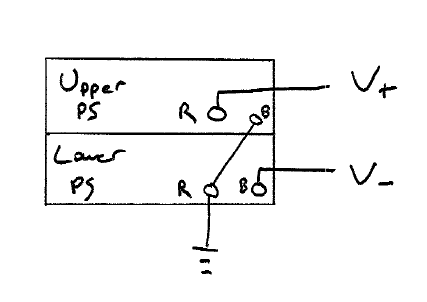
\includegraphics[height=0.30\textheight]{figs/racks.png}}  
\end{center}
\caption{\label{fig:crates} Two powersupplies ganged together to provide a postive and negative supply voltage.}
\end{figure}

You are now ready to connect your thermoelectric (TE) device! 
The TE device requires more current than your protoboard or Arduino can supply,
so each lab setup includes two 3 A power supplies.  These supplies are ganged
together (see Fig.~\ref{fig:crates}) with the positive output of LOWER supply
connectd to the negative output of the UPPER,and to the ground of your
proto-board.  With this arrangement, the postive (red) output of UPPER supply
provides a POSIVE voltage relative to ground, while the negative (black) output
of the LOWER supply provides a NEGATIVE volrage relative to ground.

Check the following:

\begin{itemize}
\item Verify that the ground connections are connections are correct.  With
nothing else connected, turn on each suply and use a multimedia to adjust the
voltage setting to $+8$ V and $-8$ V.  Make sure that your multimedia is
grounded to the protoboard ground and confirm that the polarity is correct!

\item Turn both supplies off.  Now connect the supplies to the TE board as
follows: Negative supply voltage to GREEN, ground to BLACK, and postive to RED.
(These should also be labeled -, ground, +).

\item Turn on the negative (LOWER) supply, and confirm that the fan located underneath
the TE turns on.  Turn on the UPPER supply.  Confirm that the current draw is
nearly zero.  Turn off both supplies.

\item Check that the 8 volt supplies are both OFF and that the measured output
  of your differential amplifier measured at point ``E'' is zero.

\end{itemize}

Next, {\em remove the short cicuit between points ``E'' and ``B''}.  This was
only for testing, do not leave the short circuit when connecting the TE module!
Connect the emitter (labled ``E'') of the TE module to point ``E'' in your
cicuit.  Connect the base (labeled ``B'') of the TE module to point ``B'' in
your circuit.  Check that the voltage measured at point ``E'' is still zero.  Do
not attempt to change this voltage while the 8 V supplies are off.

If you did everything correctly so far, you are probably NOT about to burn out a
power transistor on the Thermoelectric (TE) module.  We'll see!  Turn on the
lower supply, check that the current is nearly zero.  Turn on the upper supply,
check the current is nearly zero.  Check that $V_E$ is still nearly zero.

Ready?  Change the manual (constant) voltage setting in the Arduino ({\tt vman})
to 1~V and upload the sketch.  Check that the $V_E$ changes to a value of around
$1.1$~V.  You should see a small current draw in the UPPER supply (less than 0.5
A) and no current in the LOWER supply.  Change the {\tt vman} to $-1$~V and
repeat.  You should see $V_E$ change to value of around $-1.1$~V and a small
current draw in the LOWER supply.

Adjust the supply voltages on your protoboard to plus and minus 9 volts. 

Now change the value of {\tt vman} between positive and negative 2~V.  Using the
the serial monitor, you should see the effect of the temperature changing: the
thermistor resistance should change, which should change the output of your
voltage divider circuit, which should change the reported voltage $V_x$ in the
serial monitor.  Some of the TE modules are wired such that the a positive value
of {\tt vman} tends to decrease $V_x$ (positive control cools the aluminum
block) while negative values of {\tt vman} tends to decrease $V_x$ (negative
control voltage warms the aluminum block).  But some modules have opposite
polarity!  Take note of the polarity of your module (does postive $\tt vman$
cool or warm your block?)

Remove the software limits on the output voltage by changing the values of {\tt
  safe\_vout\_max} and {\tt safe\_vout\_min} to +5 V and -5 V.  Now, stepping up
in units of 1 V, check the current draw at each voltage setting and make sure
that you (1) only draw from one supply at a time, and (2) only draw up to around
1 A of current all the way to 5 V.

\section{Automatic Control}

The Arduino sketch includes a simple themometer mode which simply turns on
heating or cooling to specified values once it falls outside the comfort range.
It keeps heating or cooling until it crosses the set point within the comfort
range, then turns off and waits.

Turn off the manual control and turn on the simple thermostat by setting {\tt manual=0} and {\tt
  thermostat=1}.  Set the cooling and heating amounts to something appropriate for your polarity.

You should be able to control the temperature of the aluminum block to within
10\% of a target temperature beween 2 and 3 volts.

Once you can achieve this, you are done with the scripted part of this lab.  You are free to leave.

Or, if you prefer, you can improve the feedback algorithm to implement a PID
algorithm, and see if you can do better.

\end{document}
